\section{Methodology \& involved technologies}

\subsection{Methodology}

\begin{frame}

	\frametitle{Methodology} 
	
	\begin{itemize}
	  \item Agile software development methodology: iterative development, frequent
	  inspection and adaptation, self-organization, etc.
	  \item Following a spiral model.
	  \item Fits properly with the researching nature of the project and the
		fact that new requirements arise continuously.
	\end{itemize}
	
	% \begin{figure}
	% 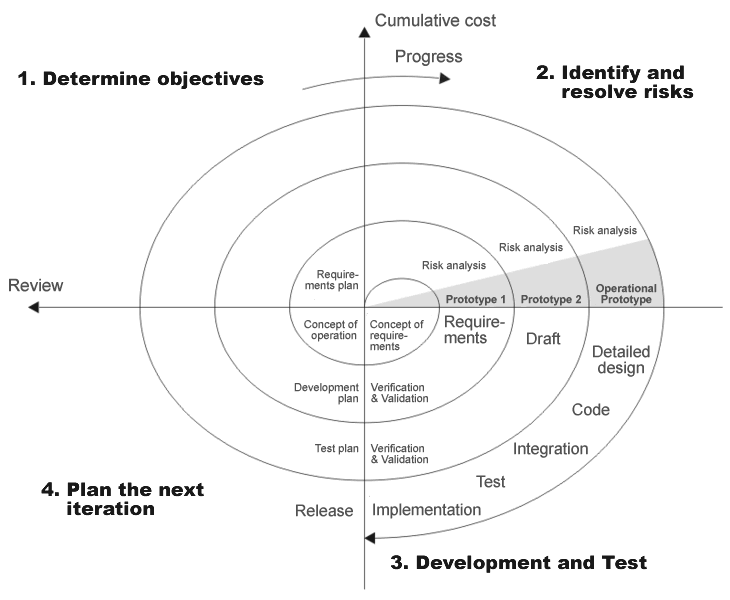
\includegraphics[scale=0.2]{img/spiral_model.png}
	% \end{figure}
	
	%\end{frame}
	
	%\begin{frame}
		\begin{table}[h]
			\tiny
			\centering
			\begin{tabular}{||r|c|c||}
			\hline \hline
			Iteration & Requirements & Affected components
			\\
			\hline
			\hline 
			1 & Share and retrieve applications & \texttt{RepositoryManager} \& \texttt{PHP
			EUT tools}\\
			\hline
			2 & Tagging & \texttt{TagManagerNode} \& \texttt{TagManagerBackEnd} \\
			\hline
			3 & Searching capabilities & \texttt{RepositoryManager},\\
			  &	\& tagging extensions &\texttt{TagManagerNode} \& \texttt{TagManagerBackEnd}\\
			\hline
			4 & GUI & \texttt{ApplicationManager} \\
			\hline \hline
			\end{tabular}
			\caption{\label{table:iterations}Iterations during the project}
		\end{table}

\end{frame}

\subsection{Involved technologies}

\begin{frame}

	\frametitle{Involved technologies} 
	
	\begin{itemize}
	  \item SOA: Service Oriented Architecture.
	  \item Paradigm for organizing and utilizing distributed
	capabilities
	  \item Resources on a network are made available
		as independent services that can be accessed without knowledge of their
		underlying platform implementation
	  \item SOAP is a lightweight protocol for exchanging structured information in
	a decentralized, distributed environment. The implementation we have used is
	Apache Axis (open source).
	\end{itemize}

\end{frame}


\begin{frame}

	\frametitle{ASTRA SOA} 
	
	\begin{itemize}
	  \item The backbone of ASTRA: the platform that offers all the services
	  (awareness, ontologies, the ones developed for this project, \ldots)
	  \item They are grouped into two subsystems: ASTRA Node and
		ASTRA Backend (Client-Server model).
	  \item Therefore it is important to distinguish between the local and remote
	  nature connection when consuming other bundles services: limitations in the
	  type of objects, problems with the network, etc.
	\end{itemize}


\end{frame}


\begin{frame}

	ASTRA SOA bundles' services used in this project:

	\begin{itemize}
	  \item \texttt{UserManager} (Backend): Manage users, their profiles 
	 and their identities.
	  \item \texttt{CommunityManager} (Backend): Connect virtual community
	  representations in within which users can share awareness information.
	  \item \texttt{AwarenessManager} (Nodes): Connection
	  between low level user-system interaction and the high level concepts related to
	  them (i.e.: rules engine kernel).
	  \item \texttt{AwarenessApplicationManager} (Nodes): Store
	  and manage local awareness applications.
	\end{itemize}


\end{frame}


\begin{frame}

	\begin{itemize}
	  \item \texttt{OntologyManager} (Nodes): Manage, look-up
	  and extend ontologies. It is executed in the Nodes.
	  \item \texttt{PersistencyManager} (Both): Storage functionalities.
	  \item \texttt{RemoteFrameworkManager} (Both): Facilities to consume remote
	  bundles services.
	  \item \texttt{EventsManager} (Both): Communicate events between bundles. 
	\end{itemize}


\end{frame}

\begin{frame}

	\frametitle{OSGi} 
	
	\begin{itemize}
	  \item OSGi (Open Services Gateway initiative) is a  flexible framework,
	  which provides a standardized environment for service deployment and operation.
	  \item The components (bundles) can be remotely installed, started, stopped,
	  updated and uninstalled without requiring a reboot.
	  \item It is a collaborative environment: bundles run in the same VM and can
	  actually share code.
	  \item It enforces a clean service oriented design approach for ASTRA, with a
	  clear distinction between interfaces and implementation.
	  \item We used OSGi-Knoplerfish implementation (BSD style license).
	\end{itemize}


\end{frame}

\begin{frame}

	\frametitle{Lucene} 
	
	\begin{itemize}
	  \item Apache Lucene is an open source information retrieval library.
	  \item It is just an indexing and search library, not an application.
	  \item It allowed us to create a search engine integrated in one of the
			bundles to offer searching capabilities in it.
	  \item It is open source, it has a great performance, it is cross-platform,
	  easily to extend, etc.
	\end{itemize}


\end{frame}


% Skipped for time limit reasons
% \begin{frame}
% 
% 	\frametitle{Other technologies involved \ldots} 
% 	
% 	\begin{itemize}
% 	  \item Java, as a main programming language.
% 	  \item Swing, widget toolkit for Java (GUI components).
% 	  \item XML, general-purpose specification for creating
% 			custom markup languages	(rules).
% 	  \item DOM, convention for representing and interacting with objects in HTML,
% 	  		XHTML and XML.
% 	  \item MySQL is a relational database management system very popular	
% 	  		in the free and open source software communities (persistency).
% 	  \item \ldots 
% 	\end{itemize}
% 
% 
% \end{frame}
